%! Author = Adham Aijou
%! Date = 20/02/2023

% Preamble
\documentclass[11pt]{article}
\usepackage{mdframed}
\usepackage[ngerman]{babel}
\usepackage[T1]{fontenc}
\usepackage[utf8]{inputenc}
\usepackage[paper=a4paper,left=40mm,right=20mm,top=25mm,bottom=20mm,footskip=25pt ]{geometry}
\usepackage[backend=biber,style=alphabetic,citestyle=alphabetic-verb]{biblatex}
\usepackage{mathptmx} %Font Times New Roman
\usepackage[toc,nonumberlist]{glossaries} %Erstellt ein Abkürzungsverzeichnis
\usepackage{array}
\usepackage{wrapfig} %Bilder können fließend in den Text eingebunden werden
\usepackage{xcolor}
\usepackage{filecontents}
\usepackage{sectsty}
\usepackage{titletoc}
\usepackage{tocvsec2}
\usepackage[title,titletoc]{appendix}
\usepackage{hyperref}
\usepackage{enumitem}
\usepackage{pgfplots}
\usepackage{tikz}
\usepackage{longtable} % Tabellen können Seitenumbrüche enthalten
\usepackage{listings} % Listings für Codebeispiele
\lstset{basicstyle=\footnotesize,
    inputencoding={utf8},
    extendedchars=false,
    language={Bash},
    escapeinside=``,
    frame = single}
\lstset{literate=%
    {Ö}{{\"O}}1
    {Ä}{{\"A}}1
    {Ü}{{\"U}}1
    {ß}{{\ss}}1
    {ü}{{\"u}}1
    {ä}{{\"a}}1
    {ö}{{\"o}}1
    {~}{{\textasciitilde}}1
}

\lstMakeShortInline[columns=fixed, basicstyle=\ttfamily\color{darkgray}]@

%\addtokomafont{disposition}{\rmfamily} %Serifenschrift für Überschriften
\counterwithout{footnote}{section} %Durchgehende Fußnoten Nummerierung
\setlength\parindent{0pt} % Einrückung für neue Absätze
\usepackage[font=footnotesize,justification = centering]{caption} %Font für Bildunterschriften
\usepackage{pifont}   % Wird für den Punkt neben den Seitzenzahlen benötigt
\usepackage[footsepline=1pt]{scrlayer-scrpage} % Anpassung von Kopf/Fußzeilen
\usepackage{setspace}
\usepackage{microtype}
% Document

\begin{document}
    \makeglossaries
    %! Author = Adham Aijou
%! Date = 20/02/2023

% Preamble
\documentclass[11pt]{article}

% Packages
\usepackage{amsmath}
\usepackage{graphicx}
\pagenumbering{Roman}
\begin{titlepage}
    \centering
%    \includegraphics[width=0.35\textwidth]{bilder/itn.jpg}\par\vspace{1cm}
    \vspace{2cm}
    Fachhochschule für die Wirtschaft Hannover \\
    - FHDW -\\
    {\scshape\Large Praxisarbeit \par}
    \vspace{1cm}
    {\huge\bfseries Ressourcen- und Terminplanung in Office365 mit Hilfe von Microsoft Graph API \par}
    \vspace{3cm}

    \normalsize{
        \begin{tabular}{l l}
            \textbf{Adham:} & \textbf{Aijou} \\
            &	Brinker Straße 72 \\
            &	30851, Langenhagen \\
            \\

            \textbf{Mentor:} & \textbf{Prof. Dr.  Ing. Klinger}\\
            \\
            \textbf{Studiengruppe:} & \textbf{HFI421IN}\\
            \\
            \textbf{Matrikelnummer:}  & \textbf{600142} \\
            \\
            \textbf{Ausbildungsbetrieb:}  & \textbf{DOOH media GmbH}\\
            & Frankenring 18\\
            & 30855 Langenhagen    \\
            \\
            \textbf{Eingereicht am:} & xx.xx.xxxx
        \end{tabular}\\
    }
    \vfill
%    \flushright \includegraphics[width=0.35\textwidth]{bilder/doohmediaLogo.png}\par\vspace{1cm}

\end{titlepage}
% Document
\begin{document}



\end{document}
    %! Author = mboehme
%! Date = 21.02.2023



% Document
    \tableofcontents
    \newpage



    %! Author = mboehme
%! Date = 21.02.2023

% Preamble

% Document

\section{Einleitung}\label{sec:einleitung}
Die Praxisarbeit befasst sich mit der Ressourcen- und Terminplanung in Office365 mithilfe von Microsoft Graph API~\cite{microsoftGraphApi}.
Die Arbeit ist in drei Teile gegliedert.
Im ersten Teil wird die Theorie der Ressourcen- und Terminplanung in Office365 mithilfe von Microsoft Graph API erläutert.
Im zweiten Teil wird die praktische Umsetzung der Theorie beschrieben.
Im dritten Teil wird die Arbeit abschließend bewertet.
    \newline
    \subsection{Fragestellungen der Arbeit}\label{subsec:fragestellungen-der-arbeit}
Die Fragestellungen der Arbeit lauten:
    \begin{itemize}
        \item Wie funktioniert die Ressourcen- und Terminplanung in Office365 mithilfe von Microsoft Graph API?
        \item Wie kann die Ressourcen- und Terminplanung in Office365 mithilfe von Microsoft Graph API praktisch umgesetzt werden?
        \item Wie kann die Arbeit abschließend bewertet werden?
    \end{itemize}
Konkret bedeutet dies:
\newline
Inwiefern und wie sinnvoll, ist der Einsatz von Microsoft Graph API für die Ressourcen- und Terminplanung in Office365, im Vergleich zu anderen APIs.
Dabei sollte berücksichtigt werden, dass dies auf den Kundenauftrag bezogen ist.
Wie sollte sowas umgesetzt werden und welche Aspekte der Microsoft Graph API sind dafür relevant?
Letztenendes soll herausgefunden werden, wie man die Arbeit quantitativ und qualitativ bewerten kann.
    \subsection{Ziele der Arbeit}\label{subsec:ziele-der-arbeit}
Die Ziele der Arbeit sind wie folgt:
    \begin{itemize}
        \item Die Theorie der Ressourcen- und Terminplanung in Office365 mithilfe von Microsoft Graph API zu erläutern.
        \item Die praktische Umsetzung der Theorie anhand eines Kundenauftrags zu beschreiben.
        \item Die Arbeit abschließend zu bewerten.
    \end{itemize}
Für die Ziele bedeutet dies, dass die Fragestellungen der Arbeit beantwortet werden müssen.
Sowohl die Theorie als auch die praktische Umsetzung der Theorie, müssen in der Arbeit beschrieben werden.
Es muss immer wieder auf die Kundenanforderungen zurückgegriffen werden.

    \subsection{Ergebnisse der Arbeit}\label{subsec:ergebnisse-der-arbeit}
Die Arbeit hat alle Ziele erreicht.
    \newglossaryentry{SPA}{name=Single Page Application (SPA), description={Eine Single Page Application (SPA) ist eine Webanwendung, die nur eine HTML-Seite besitzt.
    Diese Seite wird beim Laden der Anwendung geladen und bleibt während der gesamten Nutzung der Anwendung bestehen.}, first={Single Page Application (SPA)}, text={SPA}, short=SPA}
%\newglossaryentry{SPA}{name=SPA, description={Eine Single Page Application (SPA) ist eine Webanwendung, die nur eine HTML-Seite besitzt.}}
%\newacronym{SPA}{SPA}{Single Page Application}
    Die Microsoft Graph API ist erfolgreich eingesetzt und die Ressourcen- und Terminplanung in Office365, mithilfe von der Microsoft Graph API, wurde erfolgreich als~\gls{SPA} umgesetzt.
\newglossaryentry{TBT}{name={Total-Blocking-Time (TBT)}, description= {Die Total-Blocking-Time (TBT) ist eine Metrik, die die Gesamtzeit misst, die eine Seite blockiert wird, bis sie interaktiv ist.},
first={Total-Blocking-Time (TBT)}, text={TBT}}

Die detaillierten Aspekte Ergebnisse der Arbeit sind in den Kapiteln~\ref{sec:ergebnis} und ~\ref{sec:technische-umsetzung} beschrieben.
Das ausformulierte Ergebnis und die Schlussfolgerung dieser, sind in Kapitel~\ref{sec:ergebnis} erläutert.
\newpage


    %! Author = mboehme
%! Date = 21.02.2023



% Document
\section{Theorie}\label{sec:theorie}

\subsection{Microsoft Graph API}\label{subsec:microsoft-graph-api}
Die Microsoft Graph API ist eine \gls{RESTful} web API, die es einem erlaubt auf Daten von Microsoft 365 und Office 365 zuzugreifen.
\newglossaryentry{RESTful}{
    name=RESTful,
    description={RESTful ist ein Synonym für Representational State Transfer. RESTful ist ein Architekturstil für die Entwicklung von Webdiensten.}
}
Mit Hilfe dieser API wurde das Projekt letztendlich umgesetzt.
Weitere standen jedoch zur Verfügung:
\begin{itemize}
    \item Microsoft Outlook API
    \item Microsoft Exchange API
    \item Microsoft SharePoint API
    \item Microsoft OneDrive API
    \item Microsoft Teams API
    \item Microsoft Power Automate
\end{itemize}
Einige dieser APIs, sind nur für bestimmte Microsoft 365 und Office 365 Abonnements verfügbar.
Die Microsoft Graph API ist jedoch für alle Abonnements verfügbar.
Zudem ist die Microsoft Graph API die einzige API, die es einem erlaubt auf alle Daten von Microsoft 365 und Office 365 zuzugreifen, da sie die meisten anderen APIs integriert.
Der wichtigste Faktor bei der Entscheidung war es jedoch, dass die Microsoft Graph API, mithilfe von Azure AD, die Authentifizierung und Autorisierung von Benutzern erlaubt. Dies ist für die Anwendung von großer Bedeutung, da es dem Benutzer ermöglicht sich mit seinem Microsoft 365 oder Office 365 Account anzumelden und somit auf seine Daten zuzugreifen.


    \input{istZustand}
    %! Author = Adham Aijou
%! Date = 22/02/2023

% Preamble
\pagebreak
\section{Vorgehensweise}\label{sec:vorgehensweise}

\subsection{Prototyp}\label{subsec:prototyp}
Erst wurde ein Prototyp mithilfe von vuejs entwickelt, basierend auf folgendem Mockup, welcher erstellt wurde bevor die Grafikdesigner ein Konzept erstellt hatten:
%Das ist Vorschlag 1. Muss in Soll-Zustand geändert werden
\par\vspace{1cm}
    \centering
    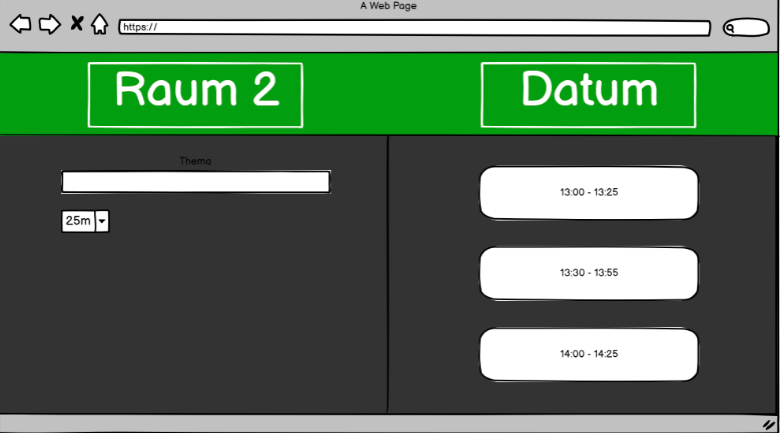
\includegraphics[width=0.8\textwidth]{Bilder/mockup}
    \caption{Mockup}
    \label{fig:Mockup}
\par\vspace{1cm}
\raggedright
    \bibliography{main}
    \bibliographystyle{plain}
    \printglossaries
\end{document}
